\documentclass{article}
\usepackage[oldvoltagedirection]{circuitikz}
\usepackage{multirow}
\usepackage{mathtools}
\usepackage[margin=0.5in]{geometry}
\pagestyle{plain}
\ctikzset{bipoles/length=2.4cm}

\begin{document}
\subsection*{DIODO}

\begin{minipage}{0.4\textwidth}
    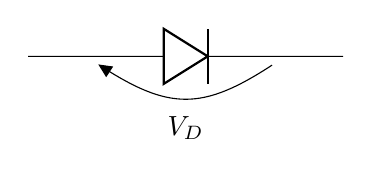
\begin{tikzpicture}
        \draw(0, 0) to[diode, v=$V_D$] (4, 0);
    \end{tikzpicture}
\end{minipage}
\begin{minipage}{0.5\textwidth}
    \[
    \begin{cases}
        I_D = 0 & \text{per} \, V_D < V_\gamma\\
        V_D = V_\gamma & \text{per}\, I_D > 0
    \end{cases}
    \]
\end{minipage}



\subsection*{BJT}
\begin{minipage}{0.4\textwidth}
    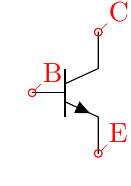
\begin{tikzpicture}
        \def\coord(#1){coordinate(#1)}
        \def\coord(#1){node[circle, red, draw, inner sep=1pt,pin={[red, overlay, inner
        sep=0.5pt,  pin distance=0.1cm, pin edge={red, overlay
        ,}]45:#1}](#1){}}

        \draw(0, 0) node[npn](tr){};
        \path(tr.B) \coord(B) (tr.E) \coord(E) (tr.C) \coord(C);
    \end{tikzpicture}
\end{minipage}
\begin{minipage}{0.5\textwidth}
    \begin{itemize}
        \item OFF
            \[ I_B = I_C = I_E = 0 \qquad\qquad \text{per} V_{BE} < V_\gamma \]

        \item AD
            \[
                \begin{aligned}
                    &V_{BE} = V_\gamma \qquad \text{per}\quad V_{CE} > V_{CE_{SAT}}\\
                    &I_C = \beta_F I_B
                \end{aligned}
            \]
        \item SAT
            \[
                \begin{aligned}
                &V_{BE} = V_\gamma \\
                &V_{CE} = V_{CE_{SAT}}
                \end{aligned} \qquad I_C < \beta_F I_B
            \]
    \end{itemize}
\end{minipage}

\bigbreak%
\subsection*{MOSFET N-MOS}

\begin{minipage}{0.4\textwidth}
    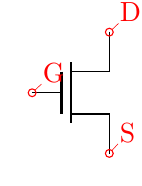
\begin{tikzpicture}
        \def\coord(#1){coordinate(#1)}
        \def\coord(#1){node[circle, red, draw, inner sep=1pt,pin={[red, overlay, inner
        sep=0.5pt,  pin distance=0.1cm, pin edge={red, overlay
        ,}]45:#1}](#1){}}

        \draw (0, 0) node[nmos](tnmos){};
        \path (tnmos.G) \coord(G)
              (tnmos.S) \coord(S)
              (tnmos.D) \coord(D);
    \end{tikzpicture}
\end{minipage}
\begin{minipage}{0.5\textwidth}
    Trasferisce uno 0 forte: $V_L = 0V$
    \begin{itemize}
        \item OFF
            \[ I_{DS} = 0 \qquad \text{per}\, V_{GS} < V_{Tn} \]
        \item SATURAZIONE
            \[ I_D  = \frac{\beta}{2} {(V_{GS} - V_{Tn})}^2 \quad\text{per}
            \begin{cases}
                V_{DS} \ge V_{GS} - V_{Tn}\\
                V_{GS} \ge V_{Tn}
            \end{cases}
        \]
        \item LINEARITÀ
            \[
                I_D = \beta\left((V_{GS} - V_T)V_{DS} - \frac{V_{DS}^2}{2}\right)
                \quad\text{per}
                \begin{cases}
                    V_{DS} < V_{GS} - V_{Tn}\\
                    V_{GS} \ge V_{Tn}
                \end{cases}
            \]
    \end{itemize}
\end{minipage}

\bigbreak%
\section*{MOSFET P-MOS}

\begin{minipage}{0.4\textwidth}
    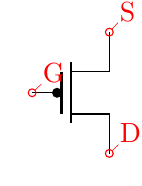
\begin{tikzpicture}
        \def\coord(#1){coordinate(#1)}
        \def\coord(#1){node[circle, red, draw, inner sep=1pt,pin={[red, overlay, inner
        sep=0.5pt,  pin distance=0.1cm, pin edge={red, overlay
        ,}]45:#1}](#1){}}

        \draw (0, 0) node[pmos](tnmos){};
        \path (tnmos.G) \coord(G)
              (tnmos.S) \coord(S)
              (tnmos.D) \coord(D);
    \end{tikzpicture}
\end{minipage}
\begin{minipage}{0.5\textwidth}
    Trasferisce 1 forte $V_H = V_{CC}$
    \begin{itemize}
        \item OFF
            \[ I_{SD} = 0 \qquad \text{per}\, V_{SG} < |V_{TP}| \]
        \item SATURAZIONE:
            \[ I_{SD} = \frac{\beta}{2}(V_{SG} - |V_{TP}|) ^2 \qquad \text{per}\,V_{SD} \ge V_{SG} - |V_{TP}| \]
        \item LINEARITÀ:
            \[
                I_{SD} = \beta\left((V_{SG} - |V_{TP}|)V_{SD} - \frac{V_{SN}^2}{2}\right)
                \qquad\text{per}
                \begin{cases}
                    V_{SD} < V_{SG} - |V_{TP}|\\
                V_{SG} \ge |V_TP|
                \end{cases}
            \]
    \end{itemize}
\end{minipage}

\end{document}
